\documentclass[border=3pt]{standalone}
\usepackage{tikz}
\usetikzlibrary{arrows.meta,calc,positioning,shapes.geometric}
\tikzset{pin/.style={-{Stealth[length=5pt]}},
  mux/.style={draw, thick, trapezium, trapezium angle=65, rotate=-90, minimum width=11mm, inner sep=1pt, font=\sffamily\scriptsize},
  preg/.style={draw, thick, fill=black!8, minimum width=3mm, minimum height=26mm}}
\begin{document}
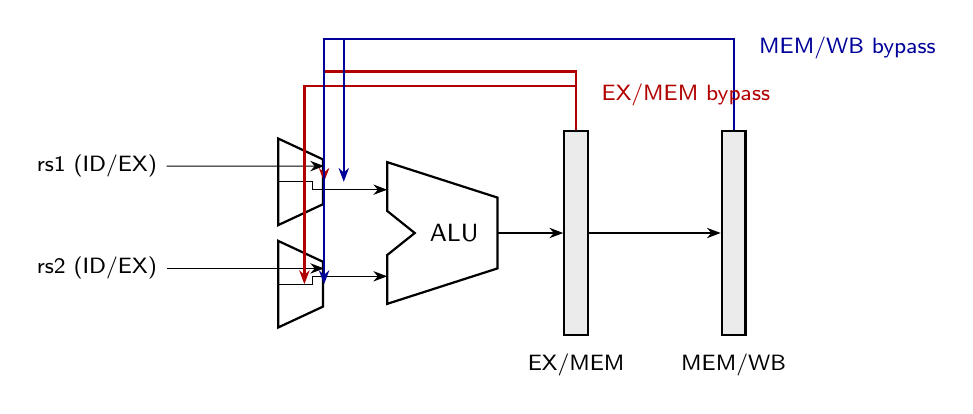
\begin{tikzpicture}[font=\sffamily\small]
  % ALU
  \draw[thick] (3.0,0.9) -- (4.4,0.45) -- (4.4,-0.45) -- (3.0,-0.9) -- (3.0,-0.28) -- (3.35,0) -- (3.0,0.28) -- cycle;
  \node[font=\sffamily\small] at (3.85,0) {ALU};
  % input muxes
  \node[mux] (m1) at (1.9,0.65) {};
  \node[mux] (m2) at (1.9,-0.65) {};
  \draw[pin] (m1.south) -- ++(0.45,0) |- (3.0,0.55);
  \draw[pin] (m2.south) -- ++(0.45,0) |- (3.0,-0.55);
  % register-file operands from ID/EX
  \draw[pin] (0.2,0.85) node[left, font=\sffamily\footnotesize]{rs1 (ID/EX)} -- ($(m1.north)+(0,0.2)$);
  \draw[pin] (0.2,-0.45) node[left, font=\sffamily\footnotesize]{rs2 (ID/EX)} -- ($(m2.north)+(0,0.2)$);
  % ALU result to EX/MEM
  \node[preg] (p3) at (5.4,0) {};
  \node[font=\sffamily\footnotesize, below=1mm of p3.south] {EX/MEM};
  \draw[pin] (4.4,0) -- (p3.west);
  \node[preg] (p4) at (7.4,0) {};
  \node[font=\sffamily\footnotesize, below=1mm of p4.south] {MEM/WB};
  \draw[pin] (p3.east) -- (p4.west);
  % bypass paths
  \draw[pin, red!70!black, thick] (5.4,1.5) -- ++(0,0.55) -| ($(m1.north)+(0,0.0)$);
  \draw[red!70!black, thick] (p3.north) -- (5.4,1.5);
  \draw[pin, red!70!black, thick] (p3.north) -- ++(0,0.55) -- ++(0,0) -| ($(m2.north)+(-0.25,0)$);
  \draw[pin, blue!60!black, thick] (p4.north) -- ++(0,1.15) -| ($(m1.north)+(0.25,0)$);
  \draw[pin, blue!60!black, thick] (p4.north) -- ++(0,1.15) -| ($(m2.north)+(0.0,0)$);
  \node[font=\sffamily\footnotesize, red!70!black, anchor=west] at (5.6,1.75) {EX/MEM bypass};
  \node[font=\sffamily\footnotesize, blue!60!black, anchor=west] at (7.6,2.35) {MEM/WB bypass};
\end{tikzpicture}
\end{document}
